% Options for packages loaded elsewhere
\PassOptionsToPackage{unicode}{hyperref}
\PassOptionsToPackage{hyphens}{url}
%
\documentclass[
  9pt,
]{article}
\usepackage{amsmath,amssymb}
\usepackage{lmodern}
\usepackage{iftex}
\ifPDFTeX
  \usepackage[T1]{fontenc}
  \usepackage[utf8]{inputenc}
  \usepackage{textcomp} % provide euro and other symbols
\else % if luatex or xetex
  \usepackage{unicode-math}
  \defaultfontfeatures{Scale=MatchLowercase}
  \defaultfontfeatures[\rmfamily]{Ligatures=TeX,Scale=1}
\fi
% Use upquote if available, for straight quotes in verbatim environments
\IfFileExists{upquote.sty}{\usepackage{upquote}}{}
\IfFileExists{microtype.sty}{% use microtype if available
  \usepackage[]{microtype}
  \UseMicrotypeSet[protrusion]{basicmath} % disable protrusion for tt fonts
}{}
\makeatletter
\@ifundefined{KOMAClassName}{% if non-KOMA class
  \IfFileExists{parskip.sty}{%
    \usepackage{parskip}
  }{% else
    \setlength{\parindent}{0pt}
    \setlength{\parskip}{6pt plus 2pt minus 1pt}}
}{% if KOMA class
  \KOMAoptions{parskip=half}}
\makeatother
\usepackage{xcolor}
\usepackage[margin=1in]{geometry}
\usepackage{color}
\usepackage{fancyvrb}
\newcommand{\VerbBar}{|}
\newcommand{\VERB}{\Verb[commandchars=\\\{\}]}
\DefineVerbatimEnvironment{Highlighting}{Verbatim}{commandchars=\\\{\}}
% Add ',fontsize=\small' for more characters per line
\usepackage{framed}
\definecolor{shadecolor}{RGB}{248,248,248}
\newenvironment{Shaded}{\begin{snugshade}}{\end{snugshade}}
\newcommand{\AlertTok}[1]{\textcolor[rgb]{0.94,0.16,0.16}{#1}}
\newcommand{\AnnotationTok}[1]{\textcolor[rgb]{0.56,0.35,0.01}{\textbf{\textit{#1}}}}
\newcommand{\AttributeTok}[1]{\textcolor[rgb]{0.77,0.63,0.00}{#1}}
\newcommand{\BaseNTok}[1]{\textcolor[rgb]{0.00,0.00,0.81}{#1}}
\newcommand{\BuiltInTok}[1]{#1}
\newcommand{\CharTok}[1]{\textcolor[rgb]{0.31,0.60,0.02}{#1}}
\newcommand{\CommentTok}[1]{\textcolor[rgb]{0.56,0.35,0.01}{\textit{#1}}}
\newcommand{\CommentVarTok}[1]{\textcolor[rgb]{0.56,0.35,0.01}{\textbf{\textit{#1}}}}
\newcommand{\ConstantTok}[1]{\textcolor[rgb]{0.00,0.00,0.00}{#1}}
\newcommand{\ControlFlowTok}[1]{\textcolor[rgb]{0.13,0.29,0.53}{\textbf{#1}}}
\newcommand{\DataTypeTok}[1]{\textcolor[rgb]{0.13,0.29,0.53}{#1}}
\newcommand{\DecValTok}[1]{\textcolor[rgb]{0.00,0.00,0.81}{#1}}
\newcommand{\DocumentationTok}[1]{\textcolor[rgb]{0.56,0.35,0.01}{\textbf{\textit{#1}}}}
\newcommand{\ErrorTok}[1]{\textcolor[rgb]{0.64,0.00,0.00}{\textbf{#1}}}
\newcommand{\ExtensionTok}[1]{#1}
\newcommand{\FloatTok}[1]{\textcolor[rgb]{0.00,0.00,0.81}{#1}}
\newcommand{\FunctionTok}[1]{\textcolor[rgb]{0.00,0.00,0.00}{#1}}
\newcommand{\ImportTok}[1]{#1}
\newcommand{\InformationTok}[1]{\textcolor[rgb]{0.56,0.35,0.01}{\textbf{\textit{#1}}}}
\newcommand{\KeywordTok}[1]{\textcolor[rgb]{0.13,0.29,0.53}{\textbf{#1}}}
\newcommand{\NormalTok}[1]{#1}
\newcommand{\OperatorTok}[1]{\textcolor[rgb]{0.81,0.36,0.00}{\textbf{#1}}}
\newcommand{\OtherTok}[1]{\textcolor[rgb]{0.56,0.35,0.01}{#1}}
\newcommand{\PreprocessorTok}[1]{\textcolor[rgb]{0.56,0.35,0.01}{\textit{#1}}}
\newcommand{\RegionMarkerTok}[1]{#1}
\newcommand{\SpecialCharTok}[1]{\textcolor[rgb]{0.00,0.00,0.00}{#1}}
\newcommand{\SpecialStringTok}[1]{\textcolor[rgb]{0.31,0.60,0.02}{#1}}
\newcommand{\StringTok}[1]{\textcolor[rgb]{0.31,0.60,0.02}{#1}}
\newcommand{\VariableTok}[1]{\textcolor[rgb]{0.00,0.00,0.00}{#1}}
\newcommand{\VerbatimStringTok}[1]{\textcolor[rgb]{0.31,0.60,0.02}{#1}}
\newcommand{\WarningTok}[1]{\textcolor[rgb]{0.56,0.35,0.01}{\textbf{\textit{#1}}}}
\usepackage{longtable,booktabs,array}
\usepackage{calc} % for calculating minipage widths
% Correct order of tables after \paragraph or \subparagraph
\usepackage{etoolbox}
\makeatletter
\patchcmd\longtable{\par}{\if@noskipsec\mbox{}\fi\par}{}{}
\makeatother
% Allow footnotes in longtable head/foot
\IfFileExists{footnotehyper.sty}{\usepackage{footnotehyper}}{\usepackage{footnote}}
\makesavenoteenv{longtable}
\usepackage{graphicx}
\makeatletter
\def\maxwidth{\ifdim\Gin@nat@width>\linewidth\linewidth\else\Gin@nat@width\fi}
\def\maxheight{\ifdim\Gin@nat@height>\textheight\textheight\else\Gin@nat@height\fi}
\makeatother
% Scale images if necessary, so that they will not overflow the page
% margins by default, and it is still possible to overwrite the defaults
% using explicit options in \includegraphics[width, height, ...]{}
\setkeys{Gin}{width=\maxwidth,height=\maxheight,keepaspectratio}
% Set default figure placement to htbp
\makeatletter
\def\fps@figure{htbp}
\makeatother
\setlength{\emergencystretch}{3em} % prevent overfull lines
\providecommand{\tightlist}{%
  \setlength{\itemsep}{0pt}\setlength{\parskip}{0pt}}
\setcounter{secnumdepth}{-\maxdimen} % remove section numbering
\newlength{\cslhangindent}
\setlength{\cslhangindent}{1.5em}
\newlength{\csllabelwidth}
\setlength{\csllabelwidth}{3em}
\newlength{\cslentryspacingunit} % times entry-spacing
\setlength{\cslentryspacingunit}{\parskip}
\newenvironment{CSLReferences}[2] % #1 hanging-ident, #2 entry spacing
 {% don't indent paragraphs
  \setlength{\parindent}{0pt}
  % turn on hanging indent if param 1 is 1
  \ifodd #1
  \let\oldpar\par
  \def\par{\hangindent=\cslhangindent\oldpar}
  \fi
  % set entry spacing
  \setlength{\parskip}{#2\cslentryspacingunit}
 }%
 {}
\usepackage{calc}
\newcommand{\CSLBlock}[1]{#1\hfill\break}
\newcommand{\CSLLeftMargin}[1]{\parbox[t]{\csllabelwidth}{#1}}
\newcommand{\CSLRightInline}[1]{\parbox[t]{\linewidth - \csllabelwidth}{#1}\break}
\newcommand{\CSLIndent}[1]{\hspace{\cslhangindent}#1}
\ifLuaTeX
\usepackage[bidi=basic]{babel}
\else
\usepackage[bidi=default]{babel}
\fi
\babelprovide[main,import]{ngerman}
% get rid of language-specific shorthands (see #6817):
\let\LanguageShortHands\languageshorthands
\def\languageshorthands#1{}
\ifLuaTeX
  \usepackage{selnolig}  % disable illegal ligatures
\fi
\IfFileExists{bookmark.sty}{\usepackage{bookmark}}{\usepackage{hyperref}}
\IfFileExists{xurl.sty}{\usepackage{xurl}}{} % add URL line breaks if available
\urlstyle{same} % disable monospaced font for URLs
\hypersetup{
  pdftitle={Pendel},
  pdfauthor={Milena Mensching, Justus Weyers},
  pdflang={de},
  hidelinks,
  pdfcreator={LaTeX via pandoc}}

\title{Pendel}
\author{Milena Mensching, Justus Weyers}
\date{2022-12-14}

\begin{document}
\maketitle

\hypertarget{versuch-1}{%
\section{Versuch 1}\label{versuch-1}}

\hypertarget{thema}{%
\subsection{Thema}\label{thema}}

Bestimmung der Wärmekapazität eines Kaloriemeters. Dieses soll in
Versuch 2 dafür verwendet werden, die spezifische Wärmekapazität zweier
Metalle zu bestimmen.

\hypertarget{versuchsaufbau-und-durchfuxfchrung}{%
\subsection{Versuchsaufbau und
Durchführung}\label{versuchsaufbau-und-durchfuxfchrung}}

\begin{figure}
\centering
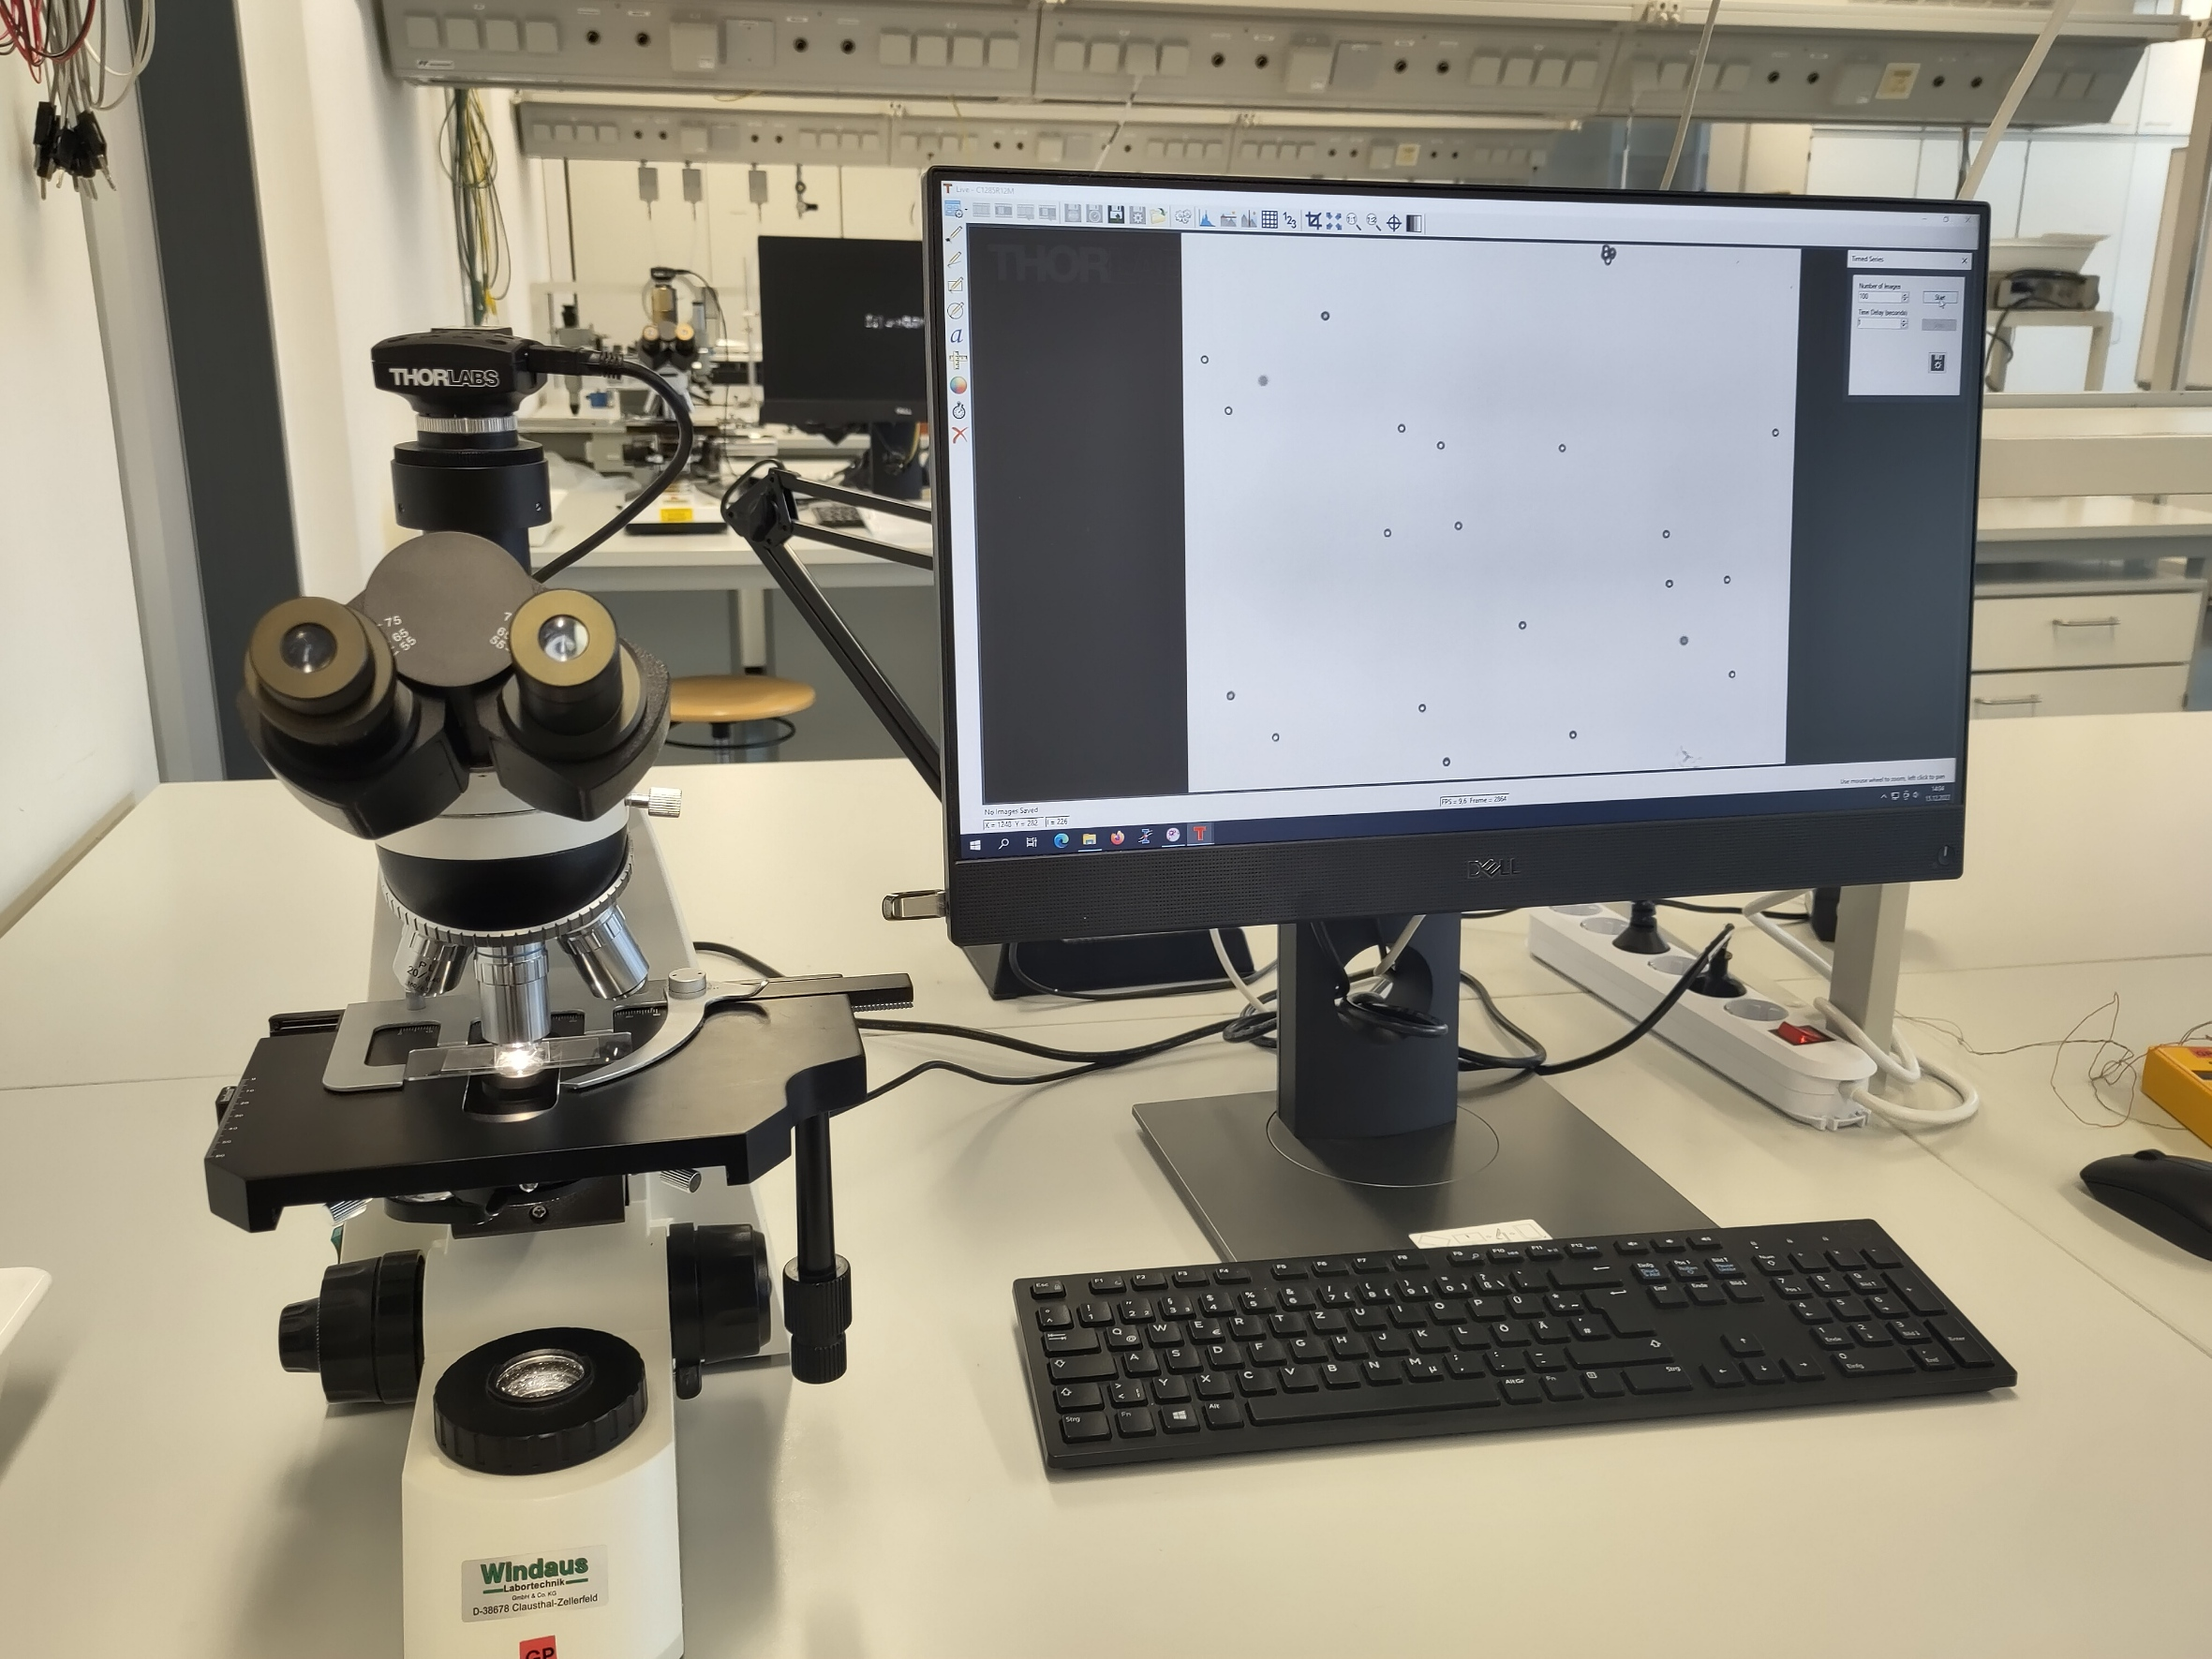
\includegraphics{"Bilder/Versuchsaufbau.png"}
\caption{Versuchsaufbau und Skizze des Schaltplans}
\end{figure}

Zu Beginn des eigentlichen Versuches wird die Raumtemperatur gemessen,
für später auftretende Fragestellungen.

Das Kaloriemeter wird leer gewogen. Im Messzylinder werden ca. \(170ml\)
destilliertes Wasser abgemessen und anschließend in das Kaloriemeter
gefüllt. In diesem Zustand wird noch einmal die Masse des nun vollen
Kaloriemeters gemessen, um die Wassermasse bestimmen zu können.

Der Deckel des Kaloriemeters mit Heizspirale, Thermometer und Rührstab
wird verschlossen. Die Heizspirale wird über Bananenstecker mit dem AC
Netzgerät verbunden. Ein Amperemeter wird in Reihe und ein Voltmeter
parallel geschaltet.

Am Netzgerät wird eine mittlere Leistung eingestellt (50\%) und über den
Zeitraum von sieben Minuten eine Temperatur-Zeit Messreihe aufgenommen.
Während der Erhitzung werden die Stromspannung und die Stromstärke
abgelesen. Diese Schwanken zwar leicht in der Zeit, jedoch immer um
einen festen Wert, welcher notiert wird.

Die steigende Innentemperatur im Kaloriemeter wird alle dreißig Sekunden
am Thermometer abgelesen und ebenfalls notiert.

\hypertarget{fehlerbetrachtung}{%
\subsection{Fehlerbetrachtung}\label{fehlerbetrachtung}}

Neben den Messunsicherheiten bei der Benutzung von Messbechern,
Multimetern und Waagen ist vorallem die Tatsachen aufzuführen, dass das
Kaloriemeter kein perfekt geschlossenes System ist. Es ist zwar
doppelwandig und luftisoliert, dannoch wirken die äußeren
Temperaturgegebeneiten auf die Innentemperatur des Kaloriemeters und
verfälschen den Erwärmungsprozess.

Die zu erstellende Temperatur-Zeitreihe unterliegt sowohl Unsicherheiten
beim Abnehmen der Temperatur zum richigen Zeitpunkt als auch der
Skalenunsicherheit des digitalen Thermometers selbst. In beiden Fällen
stellen sich die Beträge der Unsicherheiten aber als vergleichsweise
klein heraus.

\hypertarget{beobachtungen}{%
\subsection{Beobachtungen}\label{beobachtungen}}

Die Wassermasse, welche sich als Differenz aus Leer- und Vollgewicht des
Kaloriemeters berechnet beträgt \((328,8-165,1)g=163,7g\). Die
Messunsicherheit ist die doppelte Skalenunsicherheit der verwendeten
digitalen Waage, also \(u_m=2\cdot \frac{0,1g}{2\sqrt{3}} = 0,029g\).

Die Spannung liegt bei \(5,70V\), die Messunsicherheit liegt bei
\(u_U=\frac{0,01V}{2\sqrt{3}}=0,0029V\). Die Stromstärke liegt bei
\(2,20A\), die Messunsicherheit \(u_A\) beträgt
\(u_A=\frac{0,01A}{2\sqrt{3}}=0,0029A\).

Die Erhitzung im Kaloriemeter zeigt folgenden Temperaturverlauf:

\begin{figure}

{\centering 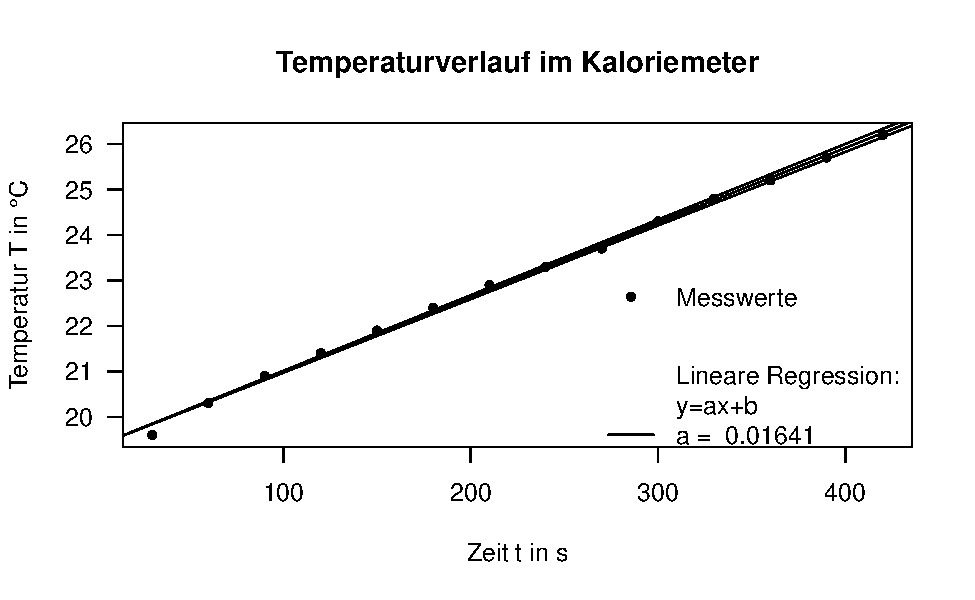
\includegraphics{Kaloriemeter_files/figure-latex/unnamed-chunk-1-1} 

}

\caption{Für sieben Minuten wurde der Temperaturverlauf der Erhitzung des Wassers im Kaloriemeter gemessen}\label{fig:unnamed-chunk-1}
\end{figure}

Die Messunsicherheiten sind augfgrund ihrer Größe nicht sichtbar. Diese
betragen für die Zeit \(u_t = \frac{0.1s}{2\sqrt{3}}=0,029s\) bzw.
\(u_T = \frac{0,1\ ^{\circ}C}{2\sqrt{3}}=0,029\ ^{\circ}C\) für die
Messunsicherheit der Temperatur.

\hypertarget{auswertung}{%
\subsection{Auswertung}\label{auswertung}}

Der Temperaturverlauf in Abbildung 1 macht im betrachteten Zeitraum
einen linearen Eindruck. Eine mittels der lm()-Funktion in R berechnete
Regressionsgerade der Form \(T(t)=A\cdot t+B\) hat die Steigung
\(a=(1641\pm 22)\cdot 10^{-5}K\ s^{-1}\):

\begin{Shaded}
\begin{Highlighting}[]
\CommentTok{\# Lineare Regression}
\NormalTok{lm }\OtherTok{\textless{}{-}} \FunctionTok{lm}\NormalTok{(zeitreiheErhitzung}\SpecialCharTok{$}\NormalTok{Temperatur}\SpecialCharTok{\textasciitilde{}}\NormalTok{zeitreiheErhitzung}\SpecialCharTok{$}\NormalTok{Zeit\_s)}
\FunctionTok{summary}\NormalTok{(lm)}
\end{Highlighting}
\end{Shaded}

\begin{verbatim}
## 
## Call:
## lm(formula = zeitreiheErhitzung$Temperatur ~ zeitreiheErhitzung$Zeit_s)
## 
## Residuals:
##      Min       1Q   Median       3Q      Max 
## -0.24286 -0.04863  0.01868  0.07830  0.10330 
## 
## Coefficients:
##                            Estimate Std. Error t value Pr(>|t|)    
## (Intercept)               1.935e+01  5.546e-02  348.90   <2e-16 ***
## zeitreiheErhitzung$Zeit_s 1.641e-02  2.171e-04   75.58   <2e-16 ***
## ---
## Signif. codes:  0 '***' 0.001 '**' 0.01 '*' 0.05 '.' 0.1 ' ' 1
## 
## Residual standard error: 0.09824 on 12 degrees of freedom
## Multiple R-squared:  0.9979, Adjusted R-squared:  0.9977 
## F-statistic:  5713 on 1 and 12 DF,  p-value: < 2.2e-16
\end{verbatim}

Für den Temperaturverlauf ist folgender Zusammenhang bekannt (o.V.
2021): \[T(t) = \frac{U\cdot I}{C_K + C_W}\cdot t + T_A\] Mit: \(C_K\):
Wärmekapazität Kaloriemeter ohne Wasser; \(C_W\): Wärmekapazität des
Wassers; \(U\): Angelegte Spannung; \(I\): Stromstärke; \(t\): Zeit;
\(T(t)\): Temperatur zum Zeitpunkt \(t\); \(T_A\): Anfangstemperatur

Wird diese Gleichung nach der Wärmekapazität des Kaloriemeters \(C_K\)
umgestellt erhält man mit der Steigung der Regressionsgeraden \(A\) für
\(C_K\): \[C_K = \frac{U*I}{A}-c_W*m_W\] Nun kann die Berechnung der
Wärmekapazität des Kaloriemeters vorgenommen werden. Dazu wird noch die
spezifische Wärmekapazität von Wasser benötigt. Diese wird im Tippler in
Tabelle 15.1 auf Seite 569 mit \(4,18 \frac{kJ}{kg\cdot K}\) angegeben
(Tipler, Mosca, und Wagner 2015).

\begin{equation*}
\begin{split}
C_K &= \frac{U*I}{A}-c_W*m_W\\
\Rightarrow &=\frac{5,70V*2,20A}{0,01641\frac{K}{s}}-4180\frac{J}{kg\cdot K}*0,1637kg\\
\underset{\text{mit VAs=J}}{\Leftrightarrow} &= 79,90219\frac{J}{K}\\
\end{split}
\end{equation*}

\begin{Shaded}
\begin{Highlighting}[]
\CommentTok{\# Berechnung der Wärmekapazität des Kaloriemeters in R}
\NormalTok{(}\FloatTok{5.7}\SpecialCharTok{*}\FloatTok{2.2}\NormalTok{)}\SpecialCharTok{/}\NormalTok{(}\FloatTok{0.01641}\NormalTok{)}\SpecialCharTok{{-}}\DecValTok{4180}\SpecialCharTok{*}\FloatTok{0.1637}
\end{Highlighting}
\end{Shaded}

\begin{verbatim}
## [1] 79.90219
\end{verbatim}

Die Messunsicherheit von \(C_K\) kann auf folgende Weise berechnet
werden:

\begin{equation*}
\begin{split}
u_{C_K} &= \sqrt{(\frac{\partial C_K}{\partial U}*u_U)^2+(\frac{\partial C_K}{\partial I}*u_I)^2+(\frac{\partial C_K}{\partial A}*u_A)^2+(\frac{\partial C_K}{\partial m_w}*u_{m_w})}\\
&=\sqrt{(\frac{I}{A}*u_U)^2+(\frac{U}{A}*u_I)^2+(\frac{U*I}{A^2}*u_A)^2+(c_w*u_{m_w})^2}\\
&= ((\frac{2,20A}{0,01641\frac{K}{s}}*0,0029V)^2+(\frac{5,70V}{0,01641\frac{K}{s}}*0,0029A)^2+(\frac{5,70V*2,20A}{(0,01641\frac{K}{s})^2}*0,00022\frac{K}{s})^2\\
&\ \ \ \ +(4180\frac{J}{kg\cdot K}*29\cdot 10^{-6}kg)^2)^{\frac{1}{2}}\\
&= 10.30224 \frac{J}{K}
\end{split}
\end{equation*}

\begin{Shaded}
\begin{Highlighting}[]
\CommentTok{\# Berechnung in R}
\FunctionTok{sqrt}\NormalTok{((}\FloatTok{2.20}\SpecialCharTok{/}\FloatTok{0.01641}\SpecialCharTok{*}\FloatTok{0.0029}\NormalTok{)}\SpecialCharTok{**}\DecValTok{2}\SpecialCharTok{+}\NormalTok{(}\FloatTok{5.70}\SpecialCharTok{/}\FloatTok{0.01641}\SpecialCharTok{*}\FloatTok{0.0029}\NormalTok{)}\SpecialCharTok{**}\DecValTok{2}\SpecialCharTok{+}
\NormalTok{       (}\FloatTok{5.70}\SpecialCharTok{*}\FloatTok{2.20}\SpecialCharTok{/}\FloatTok{0.01641}\SpecialCharTok{**}\DecValTok{2}\SpecialCharTok{*}\FloatTok{0.00022}\NormalTok{)}\SpecialCharTok{**}\DecValTok{2}\SpecialCharTok{+}\NormalTok{(}\DecValTok{4180}\SpecialCharTok{*}\DecValTok{29}\SpecialCharTok{*}\DecValTok{10}\SpecialCharTok{**}\NormalTok{(}\SpecialCharTok{{-}}\DecValTok{6}\NormalTok{))}\SpecialCharTok{**}\DecValTok{2}\NormalTok{)}
\end{Highlighting}
\end{Shaded}

\begin{verbatim}
## [1] 10.30224
\end{verbatim}

Damit wurde eine Wärmekapazität des Kaloriemeters von
\(C_K=(80 \pm 10)\frac{J}{K}\) festgestellt. Das Ergebnis ist mit einer
vergleichsweise hohen Unsicherheit behaftet.

\hypertarget{versuch-2}{%
\section{Versuch 2}\label{versuch-2}}

\hypertarget{thema-1}{%
\subsection{Thema}\label{thema-1}}

Dieser Versuch baut auf dem vorherigen Versuch 1 auf. Es soll die
spezifische Wärmekapazität zweier Metalle bestimmt werden, wofür die in
Versuch 1 ermittelte Wärmekapazität des Kaloriemeters \(C_K\) benötigt
wird. Diese wurde als \(C_K=(80 \pm 10)\frac{J}{K}\) bestimmt. Im
Kaloriemeter soll durch die Herstellung einer Mischtemperatur \(T_M\)
zwischen, auf eine Anfangstemperatur \(T_A\), erwärmtem Wasser und einem
Metall auf Raumtemperatur \(T_B\) die materialspezifische Wärmekapazität
bestimmt und so auf die Metallart geschlossen werden.

\hypertarget{versuchsaufbau}{%
\subsection{Versuchsaufbau}\label{versuchsaufbau}}

\begin{figure}
\centering
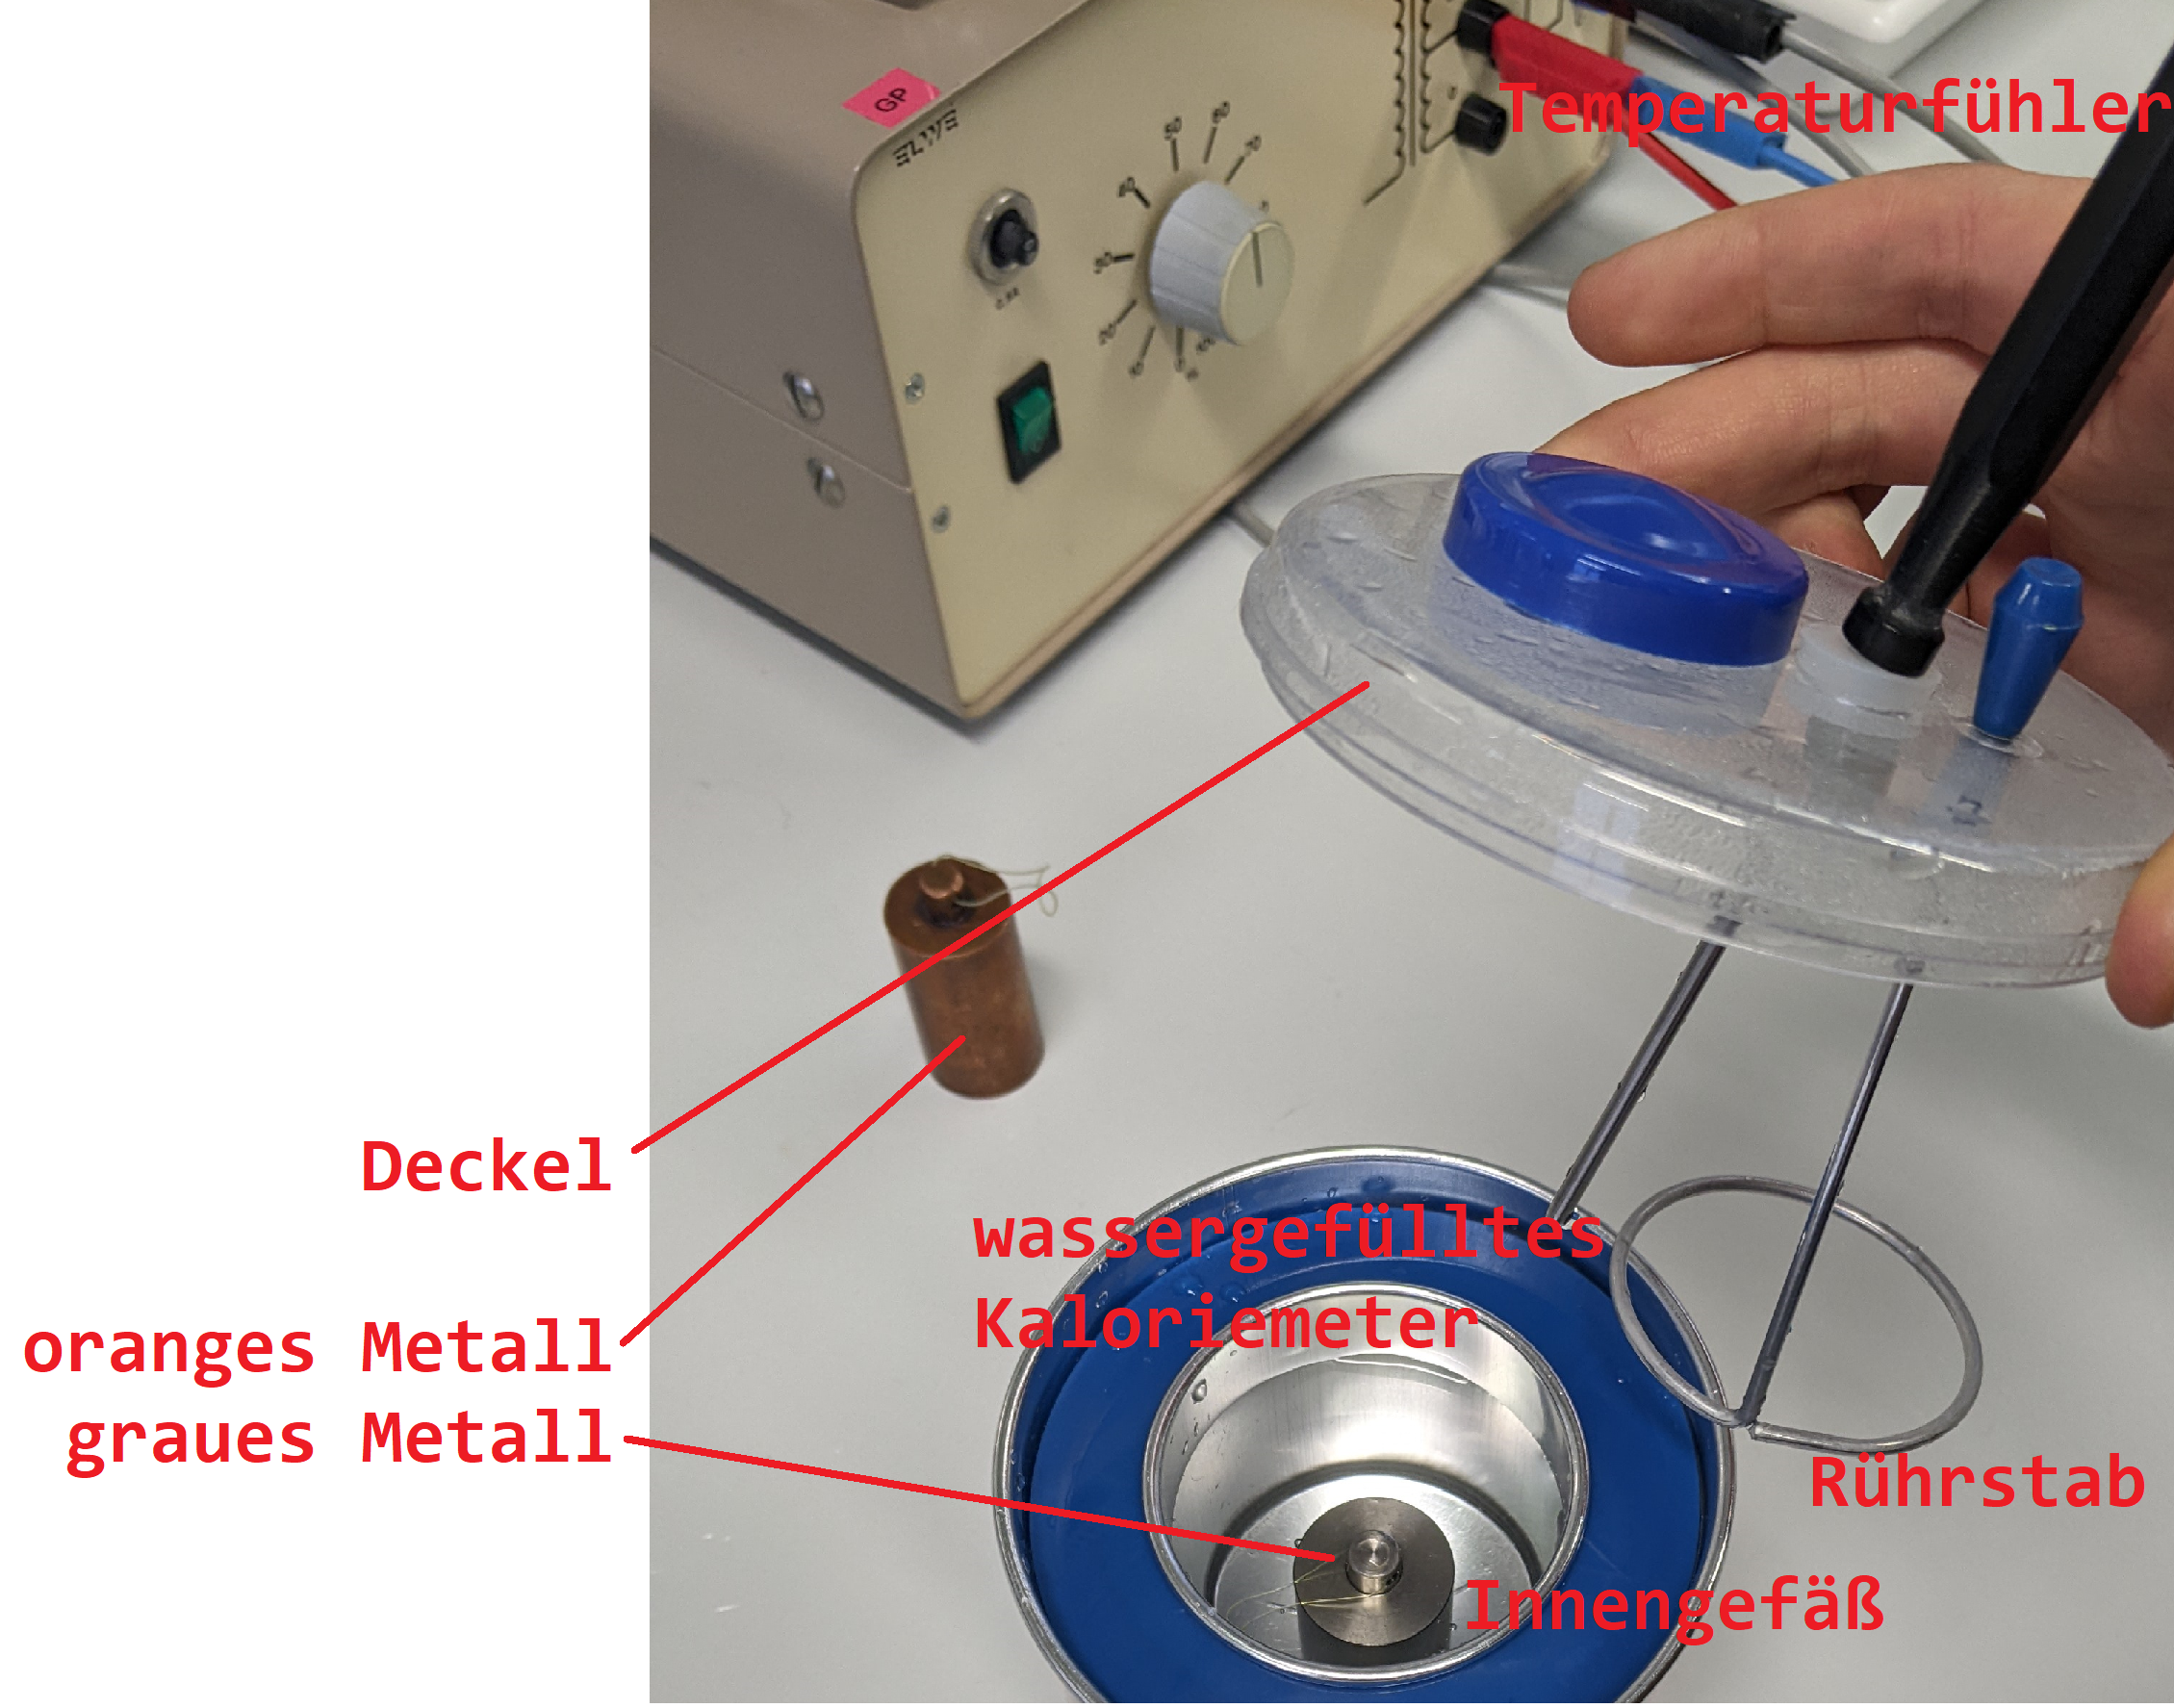
\includegraphics[width=\textwidth,height=0.25\textheight]{Bilder/V2.png}
\caption{Das mit Wasser und einem Metallzylinder gefüllte Kaloriemeter}
\end{figure}

Wasser wird auf einer Heizplatte auf ca. 50°C erwärmt. Dann wird das
Thermometer in den Deckel des Kaloriemeters gesteckt, das Wasser
eingefüllt, der Deckel geschlossen und \(T_A\) am Thermometer abgelesen.
Für das zweite Metall wird im Anschluss an den ersten Durchgang mit dem
ersten Metall wird auf gleiche Weise verfahren.

\hypertarget{fehlerbetrachtung-1}{%
\subsection{Fehlerbetrachtung}\label{fehlerbetrachtung-1}}

Viel mehr noch, als in Versuch 1, ist der Wärmeverlust während des
Versuches eine Fehlerquelle. Dies ist bedingt durch den starken
Temperaturgradienten von ca. \(30K\) zwischen der Innentemperatur des
Kaloriemeters und der Raumtemperatur, welche bei ca. 20°C lag. Der darum
hohe Wärmeabfluss aus dem Kaloriemeter ist besoonders am Deckel
bemerkbar, welcher sich während des Versuches spürbar erwärmte.

Unter anderem dieser Effekt führte dazu, dass es keinen eindeutig
bestimmbaren Wert für die Mischtemperatur im Kaloriemeter gab.
Stattdessen fiel der Temperaturwert stetig. Es wurde dann ein Wert
notiert, der, um den steigenden Einfluss des Wärmeverlustes klein zu
halten, zu einem Zeitpukt abgelesen wurde, als sich die
Temperaturabnahme im Kaloriemeter deutlich verlangsamte.

Eventuell wäre eine Erwärmung des Wassers auf z.B. 30°C für den Versuch
ausreichend gewesen und hätte bessere Ergebnisse geliefert, aufgrund der
dann geringeren Wärmeabgabe des Kaloriemeters.

Weitere Fehlerquellen sind Messunsicherheiten, welche im Gegensatz zum
Wärmeverlust aber in den folgenden Fehlerrechnungen berücksichtigt
werden.

\hypertarget{durchfuxfchrung}{%
\subsection{Durchführung}\label{durchfuxfchrung}}

Die zwei Metalle werden nacheinander untersucht. Zuerst ein
kupferfarbenes, im Vergleich schwereres Metall, als zweites ein
aluminiumgraues, leichteres Metall.

Die Volumenbestimmung der Metallzylinder erfolgte über die Bestimmung
der Wasserverdrängung in einem Standzylinder.

Da die Metallzylinder gut \(20ml\) Volumen einnahmen, wurden im
Becherglas wurden für jeden Versuch ca. \(150ml\) Wasser abgemessen, um
das Kaloriemeter mit ca. 170ml ausreichend zu füllen. Die Bestimmung der
verwendeten Wassermasse erfolgte dann durch Abwiegen des vollen und des
leeren Becherglases und durch anschließendes Subtrahieren der beiden
Werte. Die Messunsicherheit der Wassermasse beträgt zweimal die
Skalenunsicherheit der verwendeten digitalen Waage, also
\(u_{m_w}=2*\frac{0,1g}{2\sqrt{3}}=0.058g\).

Nach der Bestimmung des Metallvolumensvolumens und der Masse das Wasser
wurde dieses im Becherglas auf etwa \(50^\circ C\) erwärmt und die
genaue Anfangstemperatur dann im Kaloriemeter gemessen. Die
Skalenunsicherheit des digitalen Thermometers lag bei
\(u_T = \frac{0.1^\circ C}{2\sqrt{3}} = 0.029^\circ C\). Die gemessene
Anfangstemperatur im Kaloriemeter betrug
\(T_A=(50,000\pm 0,029)^\circ C\).

Der erste Metallzylinder wurde dann in das Kaloriemeter gestellt und die
Temperaturabnahme auf dem Thermometer verfolgt.

Für das zweite Metall wurde im Anschluss auf gleiche Weise verfahren.

\hypertarget{beobachtungen-1}{%
\subsection{Beobachtungen}\label{beobachtungen-1}}

Zur Berechnung der Unsicherheiten wurden die Skalenungenauigkeiten mit
folgenden Formeln bestimmt:

\begin{itemize}
  \item Digitale Anzeigen: $\frac{a}{2\sqrt{3}}$
  \item Analoge Anzeigen: $\frac{a}{2\sqrt{6}}$
\end{itemize}

Folgendes wurde für die zwei Metalle bestimmt:

\begin{longtable}[]{@{}
  >{\raggedright\arraybackslash}p{(\columnwidth - 10\tabcolsep) * \real{0.3023}}
  >{\raggedleft\arraybackslash}p{(\columnwidth - 10\tabcolsep) * \real{0.1047}}
  >{\raggedright\arraybackslash}p{(\columnwidth - 10\tabcolsep) * \real{0.1628}}
  >{\raggedright\arraybackslash}p{(\columnwidth - 10\tabcolsep) * \real{0.1163}}
  >{\raggedright\arraybackslash}p{(\columnwidth - 10\tabcolsep) * \real{0.1628}}
  >{\raggedleft\arraybackslash}p{(\columnwidth - 10\tabcolsep) * \real{0.1512}}@{}}
\caption{Aufgenommene Messwerte samt Unsicherheiten für das untersuchte
orangene Metall}\tabularnewline
\toprule()
\begin{minipage}[b]{\linewidth}\raggedright
\end{minipage} & \begin{minipage}[b]{\linewidth}\raggedleft
Messwert
\end{minipage} & \begin{minipage}[b]{\linewidth}\raggedright
Formelzeichen
\end{minipage} & \begin{minipage}[b]{\linewidth}\raggedright
Geräteart
\end{minipage} & \begin{minipage}[b]{\linewidth}\raggedright
Skaleneinheit
\end{minipage} & \begin{minipage}[b]{\linewidth}\raggedleft
Unsicherheit
\end{minipage} \\
\midrule()
\endfirsthead
\toprule()
\begin{minipage}[b]{\linewidth}\raggedright
\end{minipage} & \begin{minipage}[b]{\linewidth}\raggedleft
Messwert
\end{minipage} & \begin{minipage}[b]{\linewidth}\raggedright
Formelzeichen
\end{minipage} & \begin{minipage}[b]{\linewidth}\raggedright
Geräteart
\end{minipage} & \begin{minipage}[b]{\linewidth}\raggedright
Skaleneinheit
\end{minipage} & \begin{minipage}[b]{\linewidth}\raggedleft
Unsicherheit
\end{minipage} \\
\midrule()
\endhead
C Kaloriemeter {[}J/K{]} & 80.00 & C\_K & - & - & 10.000 \\
Becherglas mit Wasser {[}g{]} & 235.50 & - & digital & 0.1 & 0.029 \\
Masse Becherglas {[}g{]} & 97.40 & - & digital & 0.1 & 0.029 \\
Wassermasse {[}g{]} & 138.10 & m\_w & - & - & 0.058 \\
Metallmasse {[}g{]} & 198.00 & m\_F & digital & 0.1 & 0.029 \\
Metallvolumen {[}ml{]} & 23.00 & V\_F & analog & 1 & 0.200 \\
Anfangstemperatur {[}°C{]} & 323.15 & T\_A & digital & 0.1 & 0.029 \\
Mischtemperatur {[}°C{]} & 317.35 & T\_M & digital & 0.1 & 0.029 \\
Raumtemperatur {[}K{]} & 293.15 & T\_B & digital & 0.1 & 0.029 \\
\bottomrule()
\end{longtable}

\begin{longtable}[]{@{}
  >{\raggedright\arraybackslash}p{(\columnwidth - 10\tabcolsep) * \real{0.3023}}
  >{\raggedleft\arraybackslash}p{(\columnwidth - 10\tabcolsep) * \real{0.1047}}
  >{\raggedright\arraybackslash}p{(\columnwidth - 10\tabcolsep) * \real{0.1628}}
  >{\raggedright\arraybackslash}p{(\columnwidth - 10\tabcolsep) * \real{0.1163}}
  >{\raggedright\arraybackslash}p{(\columnwidth - 10\tabcolsep) * \real{0.1628}}
  >{\raggedleft\arraybackslash}p{(\columnwidth - 10\tabcolsep) * \real{0.1512}}@{}}
\caption{Aufgenommene Messwerte samt Unsicherheiten für das untersuchte
graue Metall}\tabularnewline
\toprule()
\begin{minipage}[b]{\linewidth}\raggedright
\end{minipage} & \begin{minipage}[b]{\linewidth}\raggedleft
Messwert
\end{minipage} & \begin{minipage}[b]{\linewidth}\raggedright
Formelzeichen
\end{minipage} & \begin{minipage}[b]{\linewidth}\raggedright
Geräteart
\end{minipage} & \begin{minipage}[b]{\linewidth}\raggedright
Skaleneinheit
\end{minipage} & \begin{minipage}[b]{\linewidth}\raggedleft
Unsicherheit
\end{minipage} \\
\midrule()
\endfirsthead
\toprule()
\begin{minipage}[b]{\linewidth}\raggedright
\end{minipage} & \begin{minipage}[b]{\linewidth}\raggedleft
Messwert
\end{minipage} & \begin{minipage}[b]{\linewidth}\raggedright
Formelzeichen
\end{minipage} & \begin{minipage}[b]{\linewidth}\raggedright
Geräteart
\end{minipage} & \begin{minipage}[b]{\linewidth}\raggedright
Skaleneinheit
\end{minipage} & \begin{minipage}[b]{\linewidth}\raggedleft
Unsicherheit
\end{minipage} \\
\midrule()
\endhead
C Kaloriemeter {[}J/K{]} & 80.00 & C\_K & - & - & 10.000 \\
Becherglas mit Wasser {[}g{]} & 241.30 & - & digital & 0.1 & 0.029 \\
Masse Becherglas {[}g{]} & 97.40 & - & digital & 0.1 & 0.029 \\
Wassermasse {[}g{]} & 143.90 & m\_w & - & - & 0.058 \\
Metallmasse {[}g{]} & 176.12 & m\_F & digital & 0.1 & 0.029 \\
Metallvolumen {[}ml{]} & 22.00 & V\_F & analog & 1 & 0.200 \\
Anfangstemperatur {[}{]} & 322.25 & T\_A & digital & 0.1 & 0.029 \\
Mischtemperatur {[}K{]} & 315.95 & T\_M & digital & 0.1 & 0.029 \\
Raumtemperatur {[}K{]} & 293.15 & T\_B & digital & 0.1 & 0.029 \\
\bottomrule()
\end{longtable}

\hypertarget{auswertung-1}{%
\subsection{Auswertung}\label{auswertung-1}}

\hypertarget{bestimmung-der-spezifischen-wuxe4rmekapazituxe4t-fuxfcr-die-zwei-metalle}{%
\subsubsection{Bestimmung der spezifischen Wärmekapazität für die zwei
Metalle}\label{bestimmung-der-spezifischen-wuxe4rmekapazituxe4t-fuxfcr-die-zwei-metalle}}

Mittels der Formel zur Berechnung der spezifischen Wärmekapazität
\(c_F\) in einem Kaloriemeter, siehe (o.V. 2021), kann nun eben diese
für beide Metalle berechnet werden.
\begin{equation}\label{Kaloriemeter:c_F}
c_F = \frac{(C_K + m_W\cdot c_W)\cdot (TM-TB)}{m_F\cdot (TA-TM)}
\end{equation}

Mit den den obigen Tabellen 1 und 2 aufgeführten Werten folgt damit für
die bestimmten Bestwerte der beiden Metalle:
\[c_F(Metall\ 1) = \frac{(80\frac{J}{K}+0,1381kg\cdot 4180\frac{J}{kg\cdot K})\cdot (317,35-293,15)K}{0,1980kg\cdot(323,15-317,35)K}\]

\begin{Shaded}
\begin{Highlighting}[]
\CommentTok{\# Berechnung in R}
\NormalTok{((}\DecValTok{80}\FloatTok{+0.1381}\SpecialCharTok{*}\DecValTok{4180}\NormalTok{)}\SpecialCharTok{*}\NormalTok{(}\FloatTok{317.35{-}293.15}\NormalTok{))}\SpecialCharTok{/}\NormalTok{(}\FloatTok{0.1980}\SpecialCharTok{*}\NormalTok{(}\FloatTok{323.15{-}317.35}\NormalTok{))}
\end{Highlighting}
\end{Shaded}

\begin{verbatim}
## [1] 13850.26
\end{verbatim}

\[c_F(Metall\ 2) = \frac{(80\frac{J}{K}+0,1439kg\cdot 4180\frac{J}{kg\cdot K})\cdot (315,95-293,15)K}{0,17612kg\cdot(322,25-315,95)K}\]

\begin{Shaded}
\begin{Highlighting}[]
\CommentTok{\# Berechnung in R}
\NormalTok{((}\DecValTok{80}\FloatTok{+0.1439}\SpecialCharTok{*}\DecValTok{4180}\NormalTok{)}\SpecialCharTok{*}\NormalTok{(}\FloatTok{315.95{-}293.15}\NormalTok{))}\SpecialCharTok{/}\NormalTok{(}\FloatTok{0.17612}\SpecialCharTok{*}\NormalTok{(}\FloatTok{322.25{-}315.95}\NormalTok{))}
\end{Highlighting}
\end{Shaded}

\begin{verbatim}
## [1] 14004.02
\end{verbatim}

Die beiden Werte sind viel zu groß.

\hypertarget{unsicherheit-der-spezifische-wuxe4rmekapazituxe4t-der-feststoffe}{%
\subsubsection{Unsicherheit der spezifische Wärmekapazität der
Feststoffe}\label{unsicherheit-der-spezifische-wuxe4rmekapazituxe4t-der-feststoffe}}

Aus Formel \ref{Kaloriemeter:c_F} kann über die Gausssche
Fehlerfortpflanzung die zugehörige Messunsicherheit \(u_{c_F}\)
berechnet werden.

\[u_{c_F}=\sqrt{(\frac{\partial c_F}{\partial C_K}*u_{C_K})^2+(\frac{\partial c_F}{\partial m_w}*u_{m_w})^2+(\frac{\partial c_F}{\partial T_M}*u_{T_M})^2+ (\frac{\partial c_F}{\partial T_B}*u_{T_B})^2+ (\frac{\partial c_F}{\partial m_F}*u_{m_F})^2+ (\frac{\partial c_F}{\partial T_A}*u_{T_A})^2}\]

\(=[(\frac{(1+m_w*c_w)*(T_M-T_B)}{m_F*(T_A-T_B)}u_{C_K})^2+(\frac{(C_K+c_w)(T_M-T_B)}{m_F(T_A-T_M)}*u_{m_w})^2+(\frac{(C_K+m_w*c_w)*(1-T_B)}{m_F(T_A-1)}*u_{T_M})^2\)
\(\ +(\frac{(C_K+m_w*c_w)*(T_M-1)}{m_F(T_A-T_M)}*u_{T_B})^2+(\frac{(C_K+m_w*c_w)*(T_M-T_B)}{T_A-T_M}*u_{m_F})^2\)
\(\ +(\frac{(C_K+m_w*c_w)*(T_M-T_B)}{m_F(1-T_M)}*u_{T_A})^2]^{\frac{1}{2}}\)

Nun können die Werte, die für die zwei Metalle ermittelt wurden
eingesetzt werden:

\hypertarget{unsicherheit-spezifische-wuxe4rmekapazituxe4t-oranges-metall}{%
\subsubsection{Unsicherheit spezifische Wärmekapazität oranges
Metall}\label{unsicherheit-spezifische-wuxe4rmekapazituxe4t-oranges-metall}}

Einsetzen in die obige Formel ergibt:

\(u_{c_F}(Metall\ 1)=[(\frac{(1+0,13810kg\cdot 4180\frac{J}{kg\cdot K})\cdot (317,35K-293,150K)}{0,19800kg\cdot (323,15K-293,150K)}\cdot 10\frac{J}{K})^2+(\frac{(80\frac{J}{K}+4180\frac{J}{kg\cdot K})(317,35K-293,150K)}{0,19800kg(323,15K-317,35K)}\cdot 0,000058kg)^2+(\frac{(80\frac{J}{K}+0,13810kg\cdot 4180\frac{J}{kg\cdot K})\cdot (1-293,150K)}{0,19800kg(323,15K-1)}\cdot 0,029K)^2+(\frac{(80\frac{J}{K}+0,13810kg\cdot 4180\frac{J}{kg\cdot K})\cdot (317,35K-1)}{0,19800kg(323,15K-317,35K)}\cdot 0,029K)^2+(\frac{(80\frac{J}{K}+0,13810kg\cdot 4180\frac{J}{kg\cdot K})\cdot (317,35K-293,150K)}{323,15K-317,35K}\cdot 0,000029kg)^2+(\frac{(80\frac{J}{K}+0,13810kg\cdot 4180\frac{J}{kg\cdot K})\cdot (317,35K-293,150K)}{0,19800kg(1-317,35K)}\cdot 0,029K)^2]^{\frac{1}{2}}\)

\newpage

\begin{Shaded}
\begin{Highlighting}[]
\CommentTok{\# Konstanten}
\NormalTok{C\_K }\OtherTok{=} \DecValTok{80} \CommentTok{\#J/kg}
\NormalTok{u\_CK }\OtherTok{=} \DecValTok{10} \CommentTok{\#J/kg}
\NormalTok{u\_mw }\OtherTok{=} \FloatTok{0.000058} \CommentTok{\#kg}
\NormalTok{u\_mF }\OtherTok{=} \FloatTok{0.000029} \CommentTok{\#kg}
\NormalTok{u\_TA }\OtherTok{=} \FloatTok{0.029} \CommentTok{\#K}
\NormalTok{u\_TB }\OtherTok{=} \FloatTok{0.029} \CommentTok{\#K}
\NormalTok{u\_TM }\OtherTok{=} \FloatTok{0.029} \CommentTok{\#K}
\NormalTok{c\_w }\OtherTok{=} \DecValTok{4180} \CommentTok{\#J}

\CommentTok{\# Variablen}
\NormalTok{m\_w }\OtherTok{=} \FloatTok{0.13810} \CommentTok{\#kg}
\NormalTok{m\_F }\OtherTok{=} \FloatTok{0.19800} \CommentTok{\#kg}
\NormalTok{T\_A }\OtherTok{=} \FloatTok{323.15} \CommentTok{\#K}
\NormalTok{T\_B }\OtherTok{=} \FloatTok{293.15} \CommentTok{\#K}
\NormalTok{T\_M }\OtherTok{=} \FloatTok{317.35} \CommentTok{\#K}

\CommentTok{\# Berechnung in R}
\FunctionTok{sqrt}\NormalTok{( ( ((}\DecValTok{1}\SpecialCharTok{+}\NormalTok{m\_w}\SpecialCharTok{*}\NormalTok{c\_w)}\SpecialCharTok{*}\NormalTok{(T\_M}\SpecialCharTok{{-}}\NormalTok{T\_B))}\SpecialCharTok{/}\NormalTok{(m\_F}\SpecialCharTok{*}\NormalTok{(T\_A}\SpecialCharTok{{-}}\NormalTok{T\_B))}\SpecialCharTok{*}\NormalTok{u\_CK)}\SpecialCharTok{**}\DecValTok{2}
     \SpecialCharTok{+}\NormalTok{( ((C\_K}\SpecialCharTok{+}\NormalTok{c\_w)}\SpecialCharTok{*}\NormalTok{(T\_M}\SpecialCharTok{{-}}\NormalTok{T\_B))}\SpecialCharTok{/}\NormalTok{(m\_F}\SpecialCharTok{*}\NormalTok{(T\_A}\SpecialCharTok{{-}}\NormalTok{T\_M))}\SpecialCharTok{*}\NormalTok{u\_mw)}\SpecialCharTok{**}\DecValTok{2}
     \SpecialCharTok{+}\NormalTok{( ((C\_K}\SpecialCharTok{+}\NormalTok{m\_w}\SpecialCharTok{*}\NormalTok{c\_w)}\SpecialCharTok{*}\NormalTok{(}\DecValTok{1}\SpecialCharTok{{-}}\NormalTok{T\_B))}\SpecialCharTok{/}\NormalTok{(m\_F}\SpecialCharTok{*}\NormalTok{(T\_A}\DecValTok{{-}1}\NormalTok{))}\SpecialCharTok{*}\NormalTok{u\_TM)}\SpecialCharTok{**}\DecValTok{2}
     \SpecialCharTok{+}\NormalTok{( ((C\_K}\SpecialCharTok{+}\NormalTok{m\_w}\SpecialCharTok{*}\NormalTok{c\_w)}\SpecialCharTok{*}\NormalTok{(T\_M}\DecValTok{{-}1}\NormalTok{))}\SpecialCharTok{/}\NormalTok{(m\_F}\SpecialCharTok{*}\NormalTok{(T\_A}\SpecialCharTok{{-}}\NormalTok{T\_M))}\SpecialCharTok{*}\NormalTok{u\_TB)}\SpecialCharTok{**}\DecValTok{2}
     \SpecialCharTok{+}\NormalTok{( ((C\_K}\SpecialCharTok{+}\NormalTok{m\_w}\SpecialCharTok{*}\NormalTok{c\_w)}\SpecialCharTok{*}\NormalTok{(T\_M}\SpecialCharTok{{-}}\NormalTok{T\_B))}\SpecialCharTok{/}\NormalTok{(T\_A}\SpecialCharTok{{-}}\NormalTok{T\_M)}\SpecialCharTok{*}\NormalTok{u\_mF)}\SpecialCharTok{**}\DecValTok{2}
     \SpecialCharTok{+}\NormalTok{( ((C\_K}\SpecialCharTok{+}\NormalTok{m\_w}\SpecialCharTok{*}\NormalTok{c\_w)}\SpecialCharTok{*}\NormalTok{(T\_M}\SpecialCharTok{{-}}\NormalTok{T\_B))}\SpecialCharTok{/}\NormalTok{(m\_F}\SpecialCharTok{*}\NormalTok{(}\DecValTok{1}\SpecialCharTok{{-}}\NormalTok{T\_M))}\SpecialCharTok{*}\NormalTok{u\_TA)}\SpecialCharTok{**}\DecValTok{2}\NormalTok{)}
\end{Highlighting}
\end{Shaded}

\begin{verbatim}
## [1] 24136.84
\end{verbatim}

\hypertarget{unsicherheit-spezifische-wuxe4rmekapazituxe4t-graues-metall}{%
\subsubsection{Unsicherheit spezifische Wärmekapazität graues
Metall}\label{unsicherheit-spezifische-wuxe4rmekapazituxe4t-graues-metall}}

\(u_{c_F}(Metall\ 2)=[(\frac{(1+0,1439kg\cdot 4180\frac{J}{kg\cdot K})\cdot (315,95K-293,150K)}{0,17612kg\cdot (322,25K-293,150K)}\cdot 10\frac{J}{K})^2+(\frac{(80\frac{J}{K}+4180\frac{J}{kg\cdot K})(315,95K-293,150K)}{0,17612kg(322,25K-315,95K)}\cdot 0,000058kg)^2+(\frac{(80\frac{J}{K}+0,1439kg\cdot 4180\frac{J}{kg\cdot K})\cdot (1-293,150K)}{0,17612kg(322,25K-1)}\cdot 0,029K)^2+(\frac{(80\frac{J}{K}+0,1439kg\cdot 4180\frac{J}{kg\cdot K})\cdot (315,95K-1)}{0,17612kg(322,25K-315,95K)}\cdot 0,029K)^2+(\frac{(80\frac{J}{K}+0,1439kg\cdot 4180\frac{J}{kg\cdot K})\cdot (315,95K-293,150K)}{322,25K-315,95K}\cdot 0,000029kg)^2+(\frac{(80\frac{J}{K}+0,1439kg\cdot 4180\frac{J}{kg\cdot K})\cdot (315,95K-293,150K)}{0,17612kg(1-315,95K)}\cdot 0,029K)^2]^{\frac{1}{2}}\)

\begin{Shaded}
\begin{Highlighting}[]
\CommentTok{\# Neudefinition Variablen}
\NormalTok{m\_w }\OtherTok{=} \FloatTok{0.14390} \CommentTok{\#kg}
\NormalTok{m\_F }\OtherTok{=} \FloatTok{0.17612} \CommentTok{\#kg}
\NormalTok{T\_A }\OtherTok{=} \FloatTok{322.25} \CommentTok{\#K}
\NormalTok{T\_B }\OtherTok{=} \FloatTok{293.15} \CommentTok{\#K}
\NormalTok{T\_M }\OtherTok{=} \FloatTok{315.95} \CommentTok{\#K}

\CommentTok{\# Berechnung in R}
\FunctionTok{sqrt}\NormalTok{( ( ((}\DecValTok{1}\SpecialCharTok{+}\NormalTok{m\_w}\SpecialCharTok{*}\NormalTok{c\_w)}\SpecialCharTok{*}\NormalTok{(T\_M}\SpecialCharTok{{-}}\NormalTok{T\_B))}\SpecialCharTok{/}\NormalTok{(m\_F}\SpecialCharTok{*}\NormalTok{(T\_A}\SpecialCharTok{{-}}\NormalTok{T\_B))}\SpecialCharTok{*}\NormalTok{u\_CK)}\SpecialCharTok{**}\DecValTok{2}
     \SpecialCharTok{+}\NormalTok{( ((C\_K}\SpecialCharTok{+}\NormalTok{c\_w)}\SpecialCharTok{*}\NormalTok{(T\_M}\SpecialCharTok{{-}}\NormalTok{T\_B))}\SpecialCharTok{/}\NormalTok{(m\_F}\SpecialCharTok{*}\NormalTok{(T\_A}\SpecialCharTok{{-}}\NormalTok{T\_M))}\SpecialCharTok{*}\NormalTok{u\_mw)}\SpecialCharTok{**}\DecValTok{2}
     \SpecialCharTok{+}\NormalTok{( ((C\_K}\SpecialCharTok{+}\NormalTok{m\_w}\SpecialCharTok{*}\NormalTok{c\_w)}\SpecialCharTok{*}\NormalTok{(}\DecValTok{1}\SpecialCharTok{{-}}\NormalTok{T\_B))}\SpecialCharTok{/}\NormalTok{(m\_F}\SpecialCharTok{*}\NormalTok{(T\_A}\DecValTok{{-}1}\NormalTok{))}\SpecialCharTok{*}\NormalTok{u\_TM)}\SpecialCharTok{**}\DecValTok{2}
     \SpecialCharTok{+}\NormalTok{( ((C\_K}\SpecialCharTok{+}\NormalTok{m\_w}\SpecialCharTok{*}\NormalTok{c\_w)}\SpecialCharTok{*}\NormalTok{(T\_M}\DecValTok{{-}1}\NormalTok{))}\SpecialCharTok{/}\NormalTok{(m\_F}\SpecialCharTok{*}\NormalTok{(T\_A}\SpecialCharTok{{-}}\NormalTok{T\_M))}\SpecialCharTok{*}\NormalTok{u\_TB)}\SpecialCharTok{**}\DecValTok{2}
     \SpecialCharTok{+}\NormalTok{( ((C\_K}\SpecialCharTok{+}\NormalTok{m\_w}\SpecialCharTok{*}\NormalTok{c\_w)}\SpecialCharTok{*}\NormalTok{(T\_M}\SpecialCharTok{{-}}\NormalTok{T\_B))}\SpecialCharTok{/}\NormalTok{(T\_A}\SpecialCharTok{{-}}\NormalTok{T\_M)}\SpecialCharTok{*}\NormalTok{u\_mF)}\SpecialCharTok{**}\DecValTok{2}
     \SpecialCharTok{+}\NormalTok{( ((C\_K}\SpecialCharTok{+}\NormalTok{m\_w}\SpecialCharTok{*}\NormalTok{c\_w)}\SpecialCharTok{*}\NormalTok{(T\_M}\SpecialCharTok{{-}}\NormalTok{T\_B))}\SpecialCharTok{/}\NormalTok{(m\_F}\SpecialCharTok{*}\NormalTok{(}\DecValTok{1}\SpecialCharTok{{-}}\NormalTok{T\_M))}\SpecialCharTok{*}\NormalTok{u\_TA)}\SpecialCharTok{**}\DecValTok{2}\NormalTok{)}
\end{Highlighting}
\end{Shaded}

\begin{verbatim}
## [1] 27384.48
\end{verbatim}

\hypertarget{interpretation}{%
\subsection{Interpretation}\label{interpretation}}

Mit den Unsicherheiten zusammengenommen wurde Folgendes bestimmt:

\begin{itemize}
  \item Metall 1: $c_F = (12\pm 24)\frac{kJ}{kg\cdot K}$
  \item Metall 2: $c_F = (14\pm 24)\frac{kJ}{kg\cdot K}$
\end{itemize}

Die Ergebnisse sind ziemlich falsch, liegen aber immerhin recht nah bei
einander und das richtige Ergebnis liegt in dem sehr großzügig
ausfallenden Fehlerintervall. Eine schnelle Recherche im Internet
liefert für die meisten Reinmetalle spezifische Wärmekapazitäten von
rund \(1\frac{kJ}{kg\cot K}\). In diese Größenordnung fällt keines der
beiden Ergebnisse, eine Aussage über die Metallart auf Basis der
Messwerte ist nicht sinnvoll. Wir tippen auf Kupfer und Aluminium.
Schließlich sind die Fehlerintervalle auch so groß, dass zu raten
seriöser erscheint.

\hypertarget{quellen}{%
\subsection*{Quellen}\label{quellen}}
\addcontentsline{toc}{subsection}{Quellen}

\hypertarget{refs}{}
\begin{CSLReferences}{1}{0}
\leavevmode\vadjust pre{\hypertarget{ref-Skript.Kaloriemeter}{}}%
o.V. 2021. \emph{Skript im Physikgrundpraktikum. T3 - Wärmekapazität}.
Universität Potsdam, Institut für Physik und Astronomie: {Universität
Potsdam}.
\url{https://moodle2.uni-potsdam.de/pluginfile.php/2512120/mod_resource/content/2/T3___W_armekapazit_at__Corona-2.pdf}.

\leavevmode\vadjust pre{\hypertarget{ref-Tipler.2015}{}}%
Tipler, Paul A., Gene Mosca, und Jenny Wagner. 2015. \emph{Physik}.
Berlin, Heidelberg: {Springer Berlin Heidelberg}.
\url{https://doi.org/10.1007/978-3-642-54166-7}.

\end{CSLReferences}

\end{document}
